En nuestra cuarta pr\'actica trabajemos con rotaciones en el espacio espectral.
Apuntamos a poder incorporar conceptos como dimensionalidad y
correlaci\'on entre bandas, que nos ayuden a utilizar mejor la informaci\'on
satelital.

Son nuestros objetivos:

\begin{itemize}
    \item Aplicar la transformada tasseled cap a una imagen multiespectral e
        interpretar el significado de cada banda.
    \item Aplicar la transformada por componentes principales a una imagen
        multiespectral e interpretar el resultado.
    \item Aplicar la transformada por componentes principales a un stack
        de bandas multiespectrales de distintas fechas e interpretar los resultados.
    \item Extraer informaci\'on de series temporales de \'indices espectrales.
\end{itemize}

\section{C\'alculo de la transformada tasseled cap para una imagen landsat}

Comencemos calculando la transformada tasseled cap para una imagen Landsat 8. \'Esta
ser\'a la primer rotaci\'on que utilizaremos en el curso cuya la
interpretaci\'on es bastante sencilla. Usaremos el paquete
\texttt{RStoolbox}.

\begin{exa}
    Para cualcular la transformada por componentes principales comenzamos
    abriendo la imagen Landsat 8 desde el metadado y convirti\'endola a reflectancia
    a tope de la cobertura, como vimos en las clases anteriores.
    \begin{lstlisting}
    xml.2016 <- readMeta("raster_data/LC82240782016304/LC82240782016304LGN00.xml")
    ref.2016 <- stackMeta(xml.2016, quantity = "sre")
    scaleF <- getMeta(ref.2016,xml.2016, what = "SCALE_FACTOR")
    ref.2016 <- ref.2016 * scaleF
    ref.2016 <- ref.2016[[-1,]]
    names(ref.2016) <- c("blue","green","red","nir","swir1","swir2")
    \end{lstlisting}

    Analizamos ahora el espacio rojo-infrarrojo cercano y rojo-verde para la imagen

    \begin{lstlisting}
    B1 <- xyplot(nir~red,data=ref.2016)
    B2 <- xyplot(red~green,data=ref.2016)
    print(B1,split=c(1,1,2,1),more=TRUE)
    print(B2,split=c(2,1,2,1),more=FALSE)
    \end{lstlisting}

    obteniendo como scatterplots (Figura \ref{fig:green-red}).

    \begin{figure}[h!]
    \begin{center}
        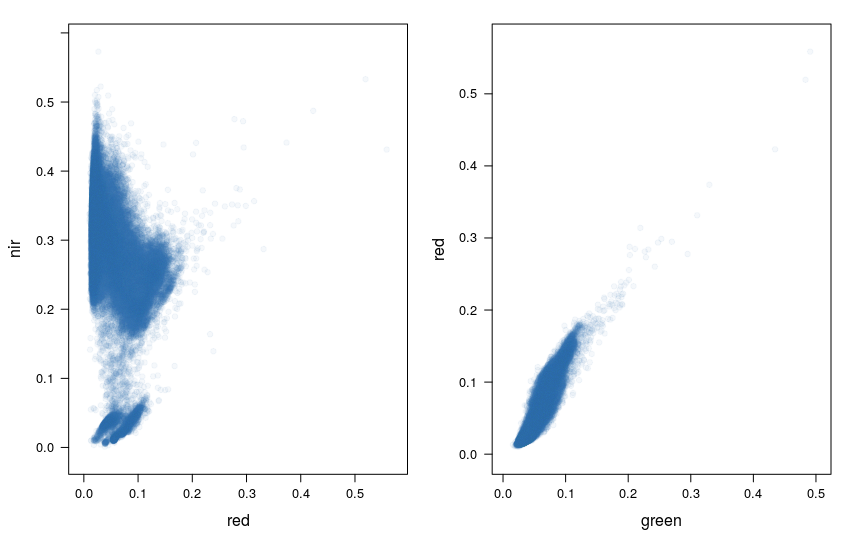
\includegraphics[scale=0.6]{red-nir-green.png}
    \end{center}
    \caption{Scatterplot verde-rojo y nir-red.}
    \label{fig:green-red}
    \end{figure}

    Calculemos ahora la transformada tasseled cap. Para eso usamos la funci\'on
    \texttt{tasseledCap} del paquete \texttt{RStoolbox}.
    \begin{lstlisting}
    tsc.2016 <- tasseledCap(ref.2016,sat="Landsat8OLI")
    \end{lstlisting}
    Tendremos una imagen de tres bandas, \emph{brillo}, \emph{verdor} y
    \emph{humedad}. Podemos graficar cada una de las bandas por separado con el
    comando \texttt{plot(tsc.2016)} o todas juntas con \texttt{plotRGB(tsc.2016,r=1,g=2,b=3, stretch="lin")}
\end{exa}

\begin{act}
    Calcule la transformada tasseled cap para la imagen Landsat 7 del año 2000.
\end{act}

\section{C\'alculo de la transformada por componentes principales}

Veamos ahora como calcular la transformada por componentes principales. Utilizaremos la
herramienta \texttt{rasterPCA} del paquete \texttt{RStoolbox}.

\begin{exa}
    Comencemos analizando la transformada por componentes principales de la
    imagen de 2016. Miremos primero los scatterplots con el comando \texttt{pairs(ref.2016)}
    obteniendolos (Figura \ref{fig:pairs2})
    \begin{figure}[h!]
    \begin{center}
        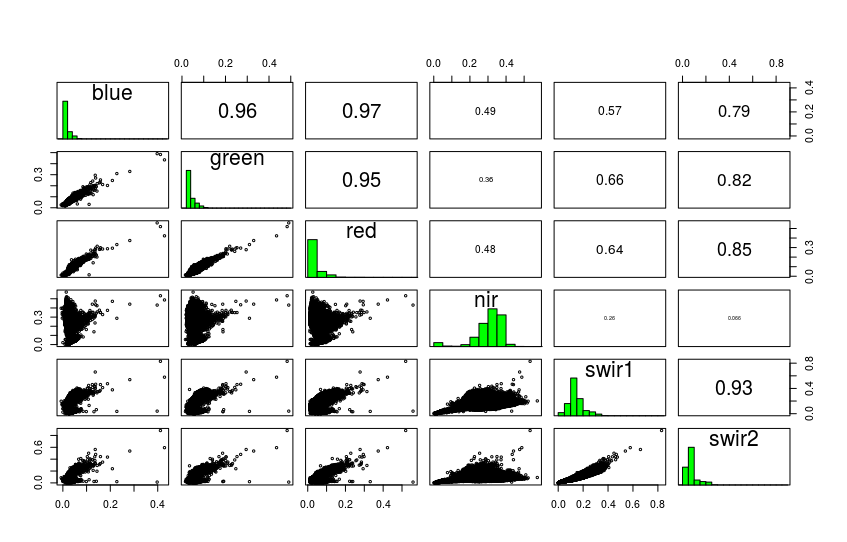
\includegraphics[scale=0.4]{pairs.png}
    \end{center}
    \caption{Scaterplots y coeficientes de correlaci\'on para la imagen Landsat 8.}
    \label{fig:pairs2}
    \end{figure}

    Mirando el resumen de la imagen vemos que hay varias bandas muy
    correlacionadas entre s\'i, como las del visible, mientras que otras lo
    estan poco, como el infrarrojo cercano y el infrarrojo de onda corta. Por lo tanto, esperamos que no
    todas las bandas sean necesarias para explicar el comportamiento de la
    imagen, al menos en el nivel de detalle m\'as bajo.

    Apliquemos entonces la transformada por componentes principales y veamos que
    sucede

    \begin{lstlisting}
        pca.2016 <- rasterPCA(ref.2016)
        summary(pca.2016$model)
    \end{lstlisting}

    El sumario del modelo obtenidos,
    \begin{Verbatim}[fontsize=\small]
    Importance of components:
                               Comp.1     Comp.2     Comp.3      Comp.4 ...
    Standard deviation     0.08079854 0.07808556 0.01242745 0.006488765 ...
    Proportion of Variance 0.50850204 0.47492732 0.01202957 0.003279516 ...
    Cumulative Proportion  0.50850204 0.98342936 0.99545892 0.998738441 ...
    \end{Verbatim}

    Al observar las varianzas, vemos que las 3 primeras explican m\'as que el
    99.5\% de la variabilidad de la imagen. Es decir que, de las 6 bandas de
    Landsat 8 en esta imagen, 3 nos alcanza para explicar casi todo el
    comportamiento. Analisemos la primera, usando el comando
    \texttt{loadings(pca.2016\$model)} para ver como son las componentes.

    \begin{Verbatim}[fontsize=\small]
    oadings:
          Comp.1  ...
    blue
    green
    red   -0.128  ...
    nir   -0.575  ...
    swir1 -0.663  ...
    swir2 -0.451  ...
    \end{Verbatim}

    La primer componente pesa siempre con el mismo signo, a
    todas las bandas. Podemos interpretarla como un
    brillo negativo y esperar que sea m\'as alta cuando miramos zonas de la imagen que
    tengan menos reflectancia en promedio. La segunda componente, presenta diferencia
    entre los valores del infrarrojo cercano y el resto de la bandas. Esta ser\'a alta
    en presencia de vegetaci\'on y baja en su ausencia. La componente tres se comporta
    de forma similar pero con las bandas del infrarrojo medio, por lo tanto podemos
    interpretarla como una componente que varia seg\'un el contenido de humedad.
\end{exa}

\begin{act}
    Calcule y analice la transformada por PCA de la imagen Landsat 7 del año
    2000.
\end{act}

\section{Algunas ideas sobre series temporales}

Empecemos esta seccion con una actividad

\begin{act}
    Aplique la transformada por componentes principales al stack de bandas del
    año 2000 y 2016.
\end{act}

Veamos que pasa al trabajar con series temporales de \'indices.

\begin{exa}
    Otra aplicaci\'on de la transformada por componentes principales
    es el an\'alisis de series temporales.
    \begin{lstlisting}
    ndvi.list <- list.files("raster_data/MOD13Q1/NDVI/", pattern = "*.tif$",
                             full.names = TRUE)
    ndvi.stack <- stack(ndvi.list)
    \end{lstlisting}
    una vez abierta la imagen la convertimos a valores entre -1 y 1 e
    interpolamos los valores faltantes.
    \begin{lstlisting}
    ndvi.stack <- ndvi.stack/1e4
    ndvi.stack <- approxNA(ndvi.stack)
    writeRaster(ndvi.stack,"ndvi-series.tif")
    \end{lstlisting}
    Una vez interpoladas las fechas donde no hab\'ia datos de NDVI, podemos
    abrirla en el QGIS y analizar distintas zonas de la imagen.

    Utilizando la herramienta de identificar objetos espaciales podemos
    consultar como es el comportamiento de la serie temporal para cada p\'ixel.

    \begin{figure}[h!]
    \begin{center}
        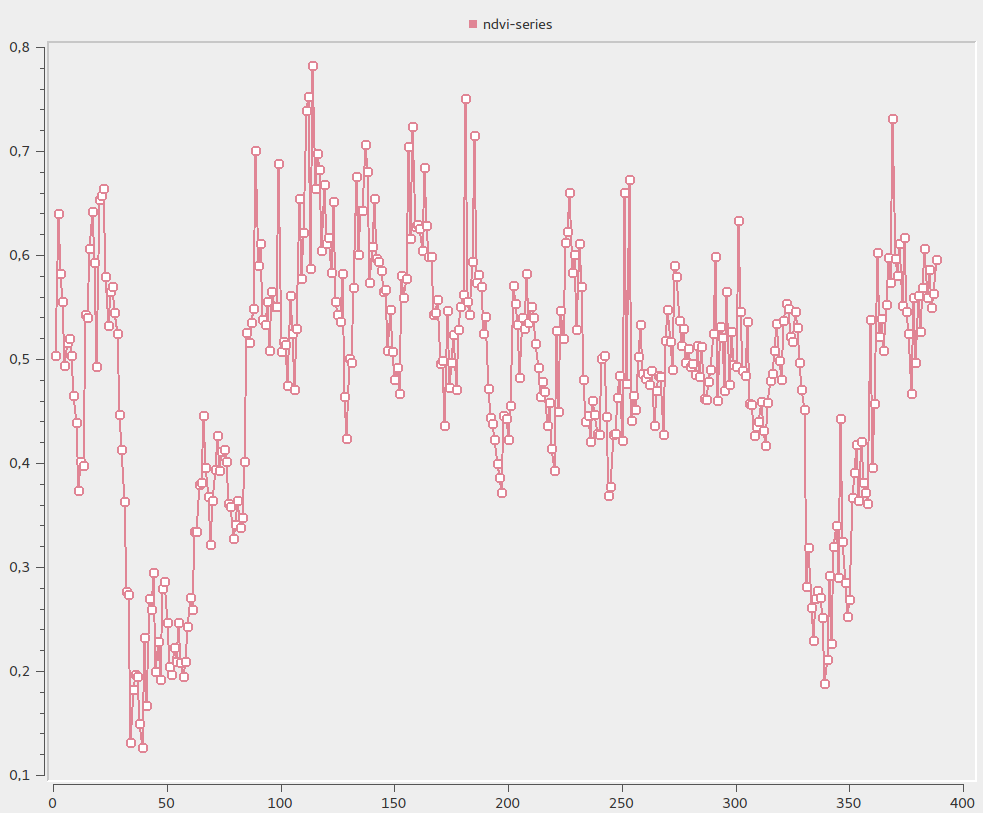
\includegraphics[scale=0.3]{series.png}
    \end{center}
    \caption{Serie temporal de valores de NDVI.}
    \label{fig:series}
    \end{figure}

    Vemos que distintas zonas tienen distintos comportamientos intra e
    interanual.

    Podemos analizar el promedio y el desv\'io standar para cada p\'ixel de la
    imagen
    \begin{lstlisting}
    ndvi.mean <- mean(ndvi.stack)
    plot(ndvi.mean)
    ndvi.sd <- calc(ndvi.stack, fun=sd)
    plot(ndvi.sd)
    \end{lstlisting}
\end{exa}


\begin{act}
    Grafique las primeras 4 componentes de la transformada por componentes
    princiales de la imagen del stack de NDVI\@. ¿Qu\'e zonas puede identificar en la
    primera? ¿Qu\'e zonas se distinguen en la segunda? ¿Qu\'e comportamiento encuentra
    en la tercera y cuarta?
\end{act}
